
\setcounter{section}{1}

\section[Quantum Review]{\hyperlink{toc}{Quantum Review}}

\begin{itemize}
    \item Harmonic oscillator distance between energy levels is always the same.
    \item wavefunctions allows for tail going past classically allowed area.
    \begin{itemize}
        \item exponential decay
    \end{itemize}
    \item \textbf{Particle in a Box (PIB)}
    \[E = \frac{n^2\hbar^2}{8mL^2}, \qquad n = 1,2,3...\]
    \[\Delta E = (2n+1) \frac{\hbar^2}{8mL^2}\]
    \item \textbf{Harmonic Oscillator (HO)}
    \[E = \hbar \omega (\frac{1}{2} + n), \qquad n=0,1,2,3...\]
    \[\Delta E = \hbar \omega\]
    
    \item \textbf{Coulomb Potential (Hydrogen 1p+1e)}
    \[ U(r) = \frac{-e^2}{4\pi \epsilon_0 r}\]
    \begin{itemize}
        \item \[\Psi(r)\Phi(\theta,\phi)\]
    \end{itemize}
    \item eigenvalues are possible energies
    \item radial quantum number $n_r = 0,1,2...$
    \item principle quantum number $n \equiv n_r + l + 1$
    \item S family orbitals (l=0)
    \item 2 types of particles that make large differences in behaviour @ $T=0$ and low $E$.
    \begin{enumerate}
        \item \textbf{Bosons:}
        \begin{itemize}
            \item occupation number can take any value 
            \item ex: photons, mesons, composite particle with integer spin (ex. Li$^7$)
            \item even total number of proton/electron/neutron
        \end{itemize}
        \item \textbf{Fermions:}
        \begin{itemize}
            \item occupation number can be zero or one (Pauli exclusion principle).
            \item ex. electrons, protons, neutrons, composite particles with half-integer spin
            \item odd number of proton/electron/neutron
        \end{itemize}
    \end{enumerate}
    \item  
    \[\beta = \frac{1}{kT}\]
    \[\bar{n}_s = \frac{1}{exp(\beta(\epsilon_s-\mu))-1}\]
    \begin{figure}
        \centering
        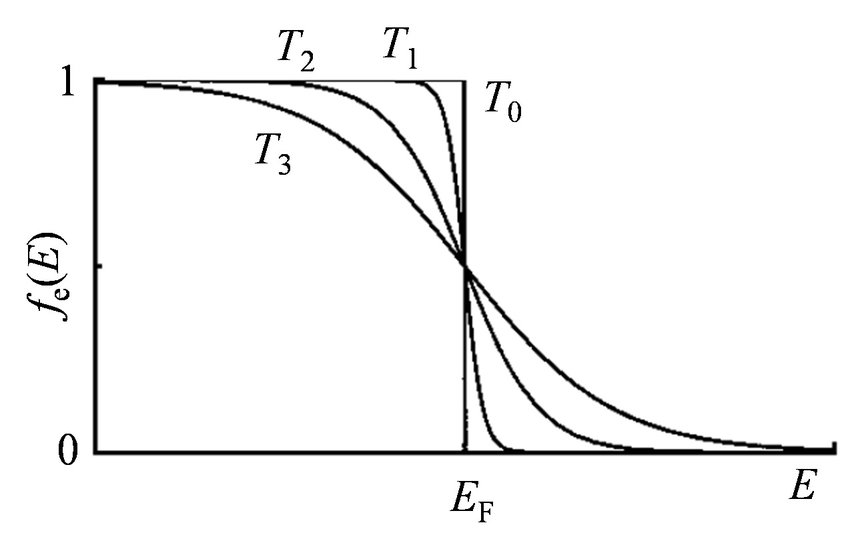
\includegraphics[width=0.5\linewidth]{Images/Fermi-Dirac-distribution.png}
        \caption{Temperature dependence of Fermi-Dirac distribution}
        \label{fig:Fermi-Dirac}
    \end{figure}
\end{itemize}
